\begin{frame}[ctb!]
\frametitle{Specific Temperature Change Calculations}
\footnotesize{A reference data set of temperature change curves was calculated. 
Repeated runs of a detailed model over the range of values in Table 
\ref{tab:thermal_cases} determined Specific Temperature Change (STC) values 
over that range.

\begin{table}[ht!]
\centering
\footnotesize{
\begin{tabular}{|l|l|l|r|}
\multicolumn{4}{c}{\textbf{Thermal Cases}}\\
\hline
\textbf{Parameter} & \textbf{Symbol} & \textbf{Units} & \textbf{Value Range} \\
\hline
Diffusivity & $\alpha_{th}$ & $[m^2\cdot s^{-1}]$ & $1.0\times10^{-7}$\\
 & & & $2.0\times10^{-7}$\\
 & & & $3.0\times10^{-7}$\\
 & & & $4.0\times10^{-7}$\\
 & & & $5.0\times10^{-7}$\\
 & & & $6.0\times10^{-7}$\\
 & & & $7.0\times10^{-7}$\\
 & & & $8.0\times10^{-7}$\\
 & & & $9.0\times10^{-7}$\\
 & & & $1.0\times10^{-6}$\\
 & & & $2.0\times10^{-6}$\\
 & & & $3.0\times10^{-6}$\\
\hline
Conductivity & $K_{th}$     & $[W\cdot m^{-1} \cdot K^{-1}]$  & $0.1, 0.5, 1, 1.5, 2, 2.5, 3, 3.5, 4, 4.5 $ \\
\hline
Spacing & $S$ & $[m]$ & 2, 5, 10, 15, 20, 25, 50 \\
\hline
Radius & $r_{lim}$ & $[m]$ & 0.1, 0.25, 0.5, 1, 2, 5 \\
\hline
Isotope & $i$ & $[-]$ & $^{241,243}Am,$  \\
        & & & $^{242,243,244,245,246}Cm,$  \\
        & & & $^{238,240,241,242}Pu$  \\
        & & & $^{134,135,137}Cs$  \\
        & & & $^{90}Sr$  \\
\hline
\end{tabular}
\caption{A thermal reference dataset of \gls{STC} values as a function of each of these parameters was generated by repeated parameterized runs of the LLNL 
MathCAD model\cite{greenberg_application_2012, greenberg_investigations_2012}.}
\label{tab:thermal_cases}
}
\end{table}


}
\end{frame}


\begin{frame}[ctb!]
\frametitle{LLNL UFD MathCAD Model}
\footnotesize{
The analytic model used to populate the reference dataset was created at 
LLNL for the UFD campaign \cite{hardin_generic_2011, 
greenberg_investigations_2012, greenberg_application_2012}. It employs an 
analytic model from Carslaw and Jaeger and is \textbf{implemented in MathCAD}
\cite{carslaw_conduction_1959, ptc_mathcad_2010}.  The integral solver in the 
MathCAD toolset is the primary calculation engine for the analytic MathCAD 
thermal model, which relies on superposition of point, finite-line, and line 
source integral solutions.  
}
\end{frame}


\begin{frame}[ctb!]
\frametitle{Scaling Demonstration}
\footnotesize{

\begin{figure}[h!]
\begin{center}
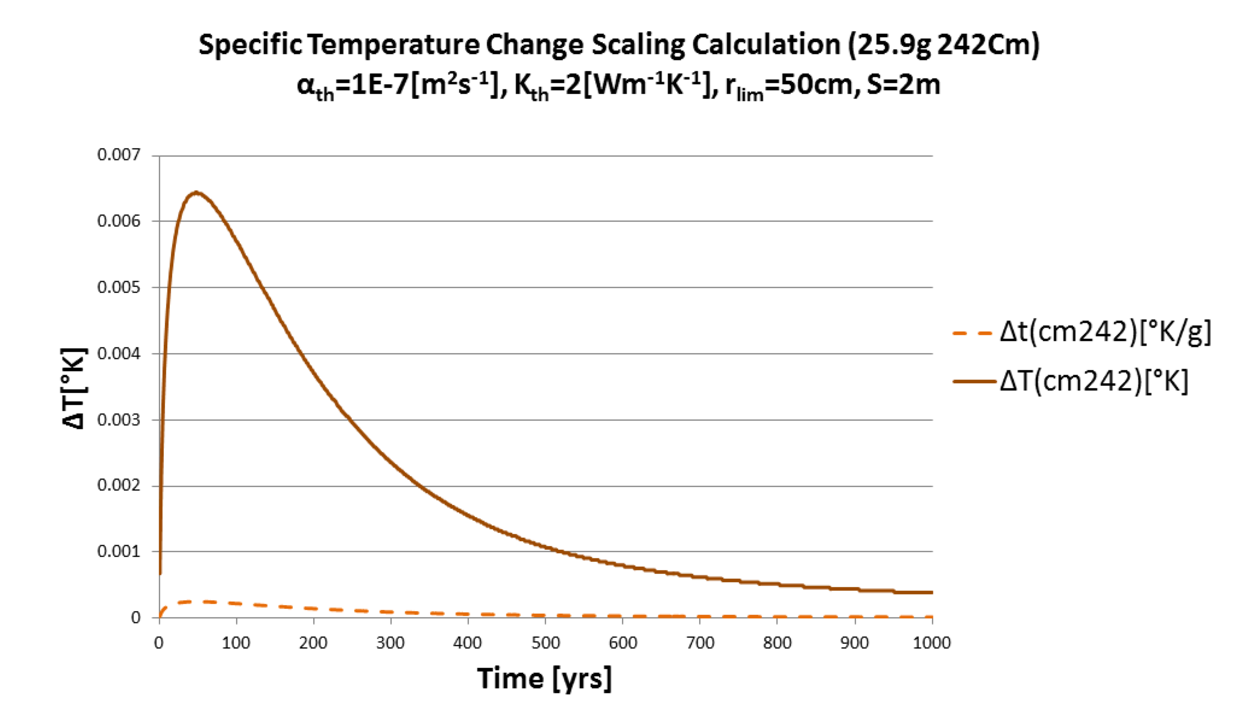
\includegraphics[width=\linewidth]{./images/CmScaling.eps}
\end{center}
\caption{As a demonstration of the calculation procedure, the temperature change 
  curve for one initial gram of $^{242}Cm$ and is scaled to represent $25.9g$, 
  approximately the $^{242}Cm$ inventory per MTHM in 51GWd burnup UOX PWR fuel. }
\label{fig:CmScaling}
\end{figure}
}
\end{frame}

\begin{frame}
\frametitle{Superposition Concept}
\footnotesize{

The supporting database was limited to some primary heat contributing isotopes 
present in traditional spent nuclear fuel, $H$, 
such that the superposition in equation \eqref{superposition} becomes 
\begin{align}
\Delta T (r_{lim},S,K_{th},\alpha_{th})&\sim \sum_{i\in H} m_i \Delta t_i(r_{lim},S,K_{th},\alpha_{th})
\label{superposition_approx}
\intertext{where}
H &= \mbox{ set of high heat isotopes }[-]\nonumber\\
S &= \mbox{ uniform waste package spacing } [m]\nonumber\\
K_{th} &= \mbox{ thermal conductivity } [W\cdot m^{-1}\cdot K^{-1}]\nonumber\\
\alpha_{th} &= \mbox{ thermal diffusivity } [m^2\cdot s^{-1}]\nonumber\\
\end{align}
}
\end{frame}


\begin{frame}
\frametitle{Superposition Demonstration}
\footnotesize{

\begin{figure}[ht!]
\begin{center}
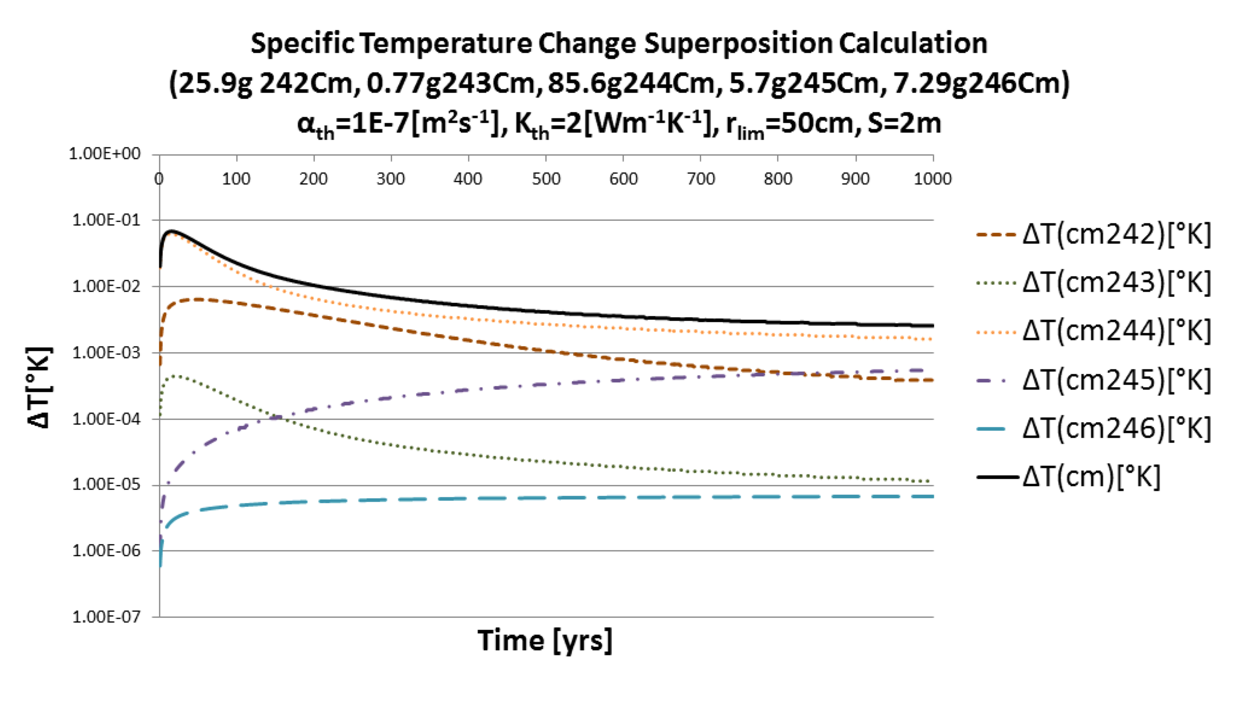
\includegraphics[width=\columnwidth]{./images/CmSuperposition.eps}
\end{center}
\caption{As a demonstration of the calculation procedure, scaled temperature change 
  curves for five curium isotopes are superimposed to achieve a total temperature 
change (note log scale).}
\label{fig:CmSuperposition}
\end{figure}

}
\end{frame}


